\documentclass{cubeamer}
\newcommand{\mcU}{\mathcal{U}}
\newcommand{\mcO}{\mathcal{O}}
\newcommand{\mcI}{\mathcal{I}}
\newcommand{\mcL}{\mathcal{L}}
\newcommand{\mcS}{\mathcal{S}}
\newcommand{\hilbert}{{\sf H}}
\newcommand{\mcB}{\mathcal{B}}
\newcommand{\mcH}{\mathcal{H}}
\newcommand{\mcF}{\mathcal{F}}
\newcommand{\mcC}{\mathcal{C}}
\newcommand{\mcT}{\mathcal{T}}
\newcommand{\mcE}{\ensuremath{\mathcal{E}} }
\newcommand{\mcG}{\ensuremath{\mathcal{G}} }
\newcommand{\mcM}{\mathcal{M}}
\newcommand{\mcN}{\mathcal{N}}
\newcommand{\nnn}{\mathcal{N}}
\newcommand{\choi}{\ensuremath{\mcD} }
\newcommand{\mmm}{\mathcal{M}}
\newcommand{\sss}{\mathcal{S}}
\newcommand{\mcD}{\mathcal{D}}
\newcommand{\mcA}{\mathcal{A}}
\newcommand{\mcP}{\mathcal{P}}
\newcommand{\Complex}{\mathbb{C}} %Para escribir al espacio de hilbert complejo
\newcommand{\Id}{\mathds{1}}% Para escribir el op. indentidad con notación chida
\newcommand{\CG}[1]{\mcC\left[#1\right]}
\newcommand{\Fuzzy}[1]{\mcF\left[#1\right]}
\title{Effective dynamics of a coarse grained system}
\subtitle{Using the maximum entropy principle}
\author[Adán Castillo Guerrero]{Adán Castillo Guerrero}
\date{April, 2022} % or whatever the date you are presenting in is
\institute[National Autonomous University of Mexico]{National Autonomous University of Mexico}
% \copyrightnotice{Published by the American Institute of Aeronautics and Astronautics, Inc., with permission}

\begin{document}

\maketitle

\cutoc
\section{Maximum entropy principle}

\begin{frame}{Classical maximum entropy state}
    \begin{columns}
        \begin{column}{0.5\textwidth}
            Supose we have access to a expected value $\expval{f(x)}$. Our task is to find the probablity density function $p(x)$ such that:
            \begin{equation*}
                \expval{f(x)}=\sum_{i}p(x_{i})f(x_{i}).
            \end{equation*}
            Such function is not unique. We choose the one that maximizes entropy.
                \begin{equation*}
                    H=-K\sum_{p}p(x_{i})\log{p(x_{i})}.
                \end{equation*}
        \end{column}
        \begin{column}{0.5\textwidth}
                Entropy is a measure of the average quantity of information. \\
                \vspace{0.2cm}
                \begin{tcolorbox}
                    Chain of characters $\{A,B,C,D\}$\\
                    If $p(x)=\frac{1}{4}$\\
                    $\rightarrow$ assign $\{00, 01, 10, 11\}$\\
                    $\rightarrow$ $2$ bits average\\
                    \\
                    If $p(x)=\{\frac{1}{2},\frac{1}{4},\frac{1}{8},\frac{1}{8}\}$\\
                    $\rightarrow$ assign $\{1, 10, 110, 111\}$\\
                    $\rightarrow$ $1.75$  bits average
                \end{tcolorbox}
        \end{column}
    \end{columns}
\end{frame}

\begin{frame}{Classical maximum entropy principle}
    \begin{columns}
        \begin{column}{0.5\textwidth}
            The entropy can be maximized by the method of the Lagrange multipliers. Use $\lambda$ and $\mu$
            along with the restriction
            \begin{equation*}
                \expval{f(x)}=\sum_{i}p(x_{i})f(x_{i}).
            \end{equation*}
            Solution is
            \begin{equation*}
                p(x_{i})=e^{-\lambda-\mu f(x_{i})}
            \end{equation*}
            That is the maximum entropy density function.
        \end{column}
        \begin{column}{0.5\textwidth}
            Notice that the only assumption made by the estimate is that of the restriction of $\expval{f(x)}$.
            \begin{itemize}
                \item The estimate doesn't need to predict measurements. It's an estimate.
                \item Little information (restrictions) leads to poor estimates.
                \item MaxEnt is the best possible estimate given a number of experimental restricions.
            \end{itemize}
        \end{column}
    \end{columns}
\end{frame}


\section{Maximum entropy state}

\begin{frame}{Quantum maximum entropy state}
    \begin{columns}
        \begin{column}{0.5\textwidth}
            Maximum entropy estimate can be extended to quantum mechanics. Given a set observables $\hat{G}_{i}$ it is possible to construct a maximum entropy state as
            \begin{equation*}
                \varrho_{max}=\frac{1}{\Tr(e^{\sum_{i}\lambda_{i}\hat{G}_{i}})}e^{\sum_{i}\lambda_{i}\hat{G}_{i}},
            \end{equation*}
            where $\lambda_{i}$ are the Lagrange multipliers used to maximize the von Neumann entropy
            \begin{equation*}
                S(\rho)=-\Tr(\rho\ln{\rho}).
            \end{equation*}
        \end{column}
        \begin{column}{0.5\textwidth}
            Because we're dealing with a coarse grained system, we do not have acces to all the observables of the system. Our coarse graining map
            \begin{equation*}
                \CG{\varrho}=\Tr_{2}(p\varrho+(1-p)S\varrho S^{\dag})
            \end{equation*}
            is of the form $\mcC:\mcS(\hilbert_{4})\rightarrow\mcS(\hilbert_{2})$. Meaning we have access to a tomographically complete set of observables in $\mcS(\hilbert_{2})$. 
        \end{column}
    \end{columns}
\end{frame}

\begin{frame}{State construction}
    \begin{columns}
        \begin{column}{0.5\textwidth}
            If we use the Pauli spin observables, $\sigma_{i}$:
            \begin{align*}
                \langle \sigma_{i}\rangle=&\Tr{\sigma_{i} \rho}\\
                =&\Tr{\sigma_{i}\otimes\Id(p\varrho+(1-p)S\varrho S)}\\
                =&\Tr{(p\sigma_{i}\otimes\Id+(1-p)\Id\otimes\sigma_{i})\varrho}\\
                =&\Tr{\hat{G}_{i}\varrho}\\
                =&\langle \hat{G}_{i}\rangle.
            \end{align*}
            We can construct $\varrho_{max}$ via
            \begin{equation*}
                \hat{G}_{i}=p\sigma_{i}\otimes\Id+(1-p)\Id\otimes\sigma_{i}.
            \end{equation*}
        \end{column}
        \begin{column}{0.5\textwidth}
            Maximum entropy state is
            \begin{equation*}
                \varrho_{max}(\rho)=\frac{1}{Z}\text{exp}(-\sum_{i}\lambda_{i}\hat{G}_{i}).
            \end{equation*}
            But may be written as
            \begin{equation*}
                \varrho_{max}=\frac{e^{-\lambda p(\hat{r}_{\rho}\cdot\vec{\sigma})}}{Z_{1}} \otimes \frac{e^{-\lambda(1-p)(\hat{r}_{\rho}\cdot\vec{\sigma})}}{Z_{2}}.
            \end{equation*}
            Where $\hat{r}_{\rho}$ is $\rho$'s unit Bloch vector, and $\lambda=\sqrt{\lambda^{2}_{1}+\lambda^{2}_{2}+\lambda^{2}_{3}}$.
        \end{column}
    \end{columns}
\end{frame}


\begin{frame}{Lagrange \textit{variable} and purity}
    \begin{columns}
        \begin{column}{0.5\textwidth}
            Having $\varrho_{max}$ in terms of $\lambda$ instead of observables is not ideal. The effective state is
            \begin{equation*}
                \rho=\frac{1}{2}(\Id+r_{\rho}\hat{r}_{\rho}\cdot\vec{\sigma}).
            \end{equation*}
            The relation between the observables and the Lagrange variable is
            \begin{equation*}
                r_{\rho}=-(p\tanh{\lambda p}+(1-p)\tanh{\lambda (1-p)}).
            \end{equation*}
            $r_{\rho}$ is realted to purity of the effective state by
            \begin{equation*}
                r_{\rho}=\sqrt{2\text{Pu}(\rho)-1}.
            \end{equation*}
        \end{column}
        \begin{column}{0.5\textwidth}
            \begin{figure}[h!]
                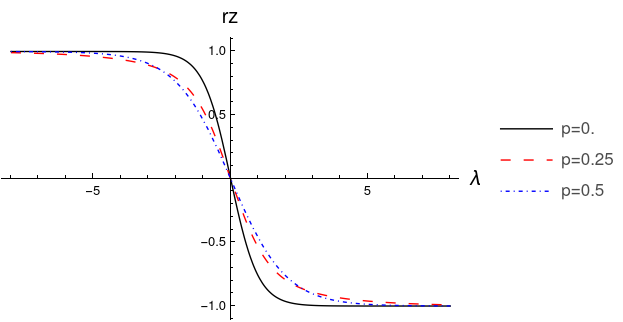
\includegraphics[width=0.8\columnwidth]{../notes/log/maxent/figures/rz(lambda)_lambda-8to8.png}%
                \caption{$r_{\rho}$ as a function of $\lambda$ for different values of $p$}
            \end{figure}
        \end{column}
    \end{columns}
\end{frame}

\section{Effective dynamics}

\begin{frame}{Dynamics in quantum mechanics}
    Closed quantum systems evolution is described by the von Neumann equation
    \begin{equation*}
        i\hbar\frac{d}{d t} \varrho(t)=[H,\rho(t)].
    \end{equation*}
    Solution being an unitary evolution operator $\mcU_{t}=e^{-iH(t)/\hbar}$ such that
    \begin{equation*}
        \varrho(t)=\mcU_{t}\varrho(0)\mcU_{t}^{\dag}.
    \end{equation*}
    We assume that the microscopic state is closed. The effective dynamics are
    \begin{equation*}
        \Gamma_{t}^{\mcM,\rho}[\rho]=(\Tr_{2}\circ\mcF\circ\mcU\circ\mcM)[\rho].
    \end{equation*}
        Here, $\mcM$ sends a coarse state $\rho$ to the compatible maximum entropy state $\varrho_{max}$.
\end{frame}

\subsection{Toy dynamics}

\begin{frame}{SWAP gate}
    State before and after the SWAP evolution is
    \begin{align*}
        \rho(0)&=\frac{1}{2}[\Id+(\hat{r}_{\rho}\cdot\vec{\sigma})(p\tanh{-\lambda p}+(1-p)\tanh{-\lambda (1-p)})],\\
        \rho(t=1)&=\frac{1}{2}[\Id+(\hat{r}_{\rho}\cdot\vec{\sigma})((1-p)\tanh{-\lambda p}+p\tanh{-\lambda (1-p)})].
        \end{align*}
    Both states have the same orientation, but different purity. The effective dynamics are described by a contraction of the Bloch sphere. Contraction factor depends on $\lambda(\rho)$:
    \begin{equation*}
        \kappa_{1}=\frac{r_{\rho(1)}}{r_{\rho(0)}}=\frac{(1-p)\tanh{\lambda p}+p\tanh{\lambda (1-p)}}{
          p\tanh{\lambda p}+(1-p)\tanh{\lambda (1-p)}}.
      \end{equation*}
      This evolution can be written as
      \begin{equation*}
        \boxed{\frac{1}{2}(\Id+\vec{r}_{\rho}\cdot\vec{\sigma}) \xrightarrow{S} \frac{1}{2}(\Id+\kappa_{1}^{\rho}\vec{r}_{\rho}\cdot\vec{\sigma})}
      \end{equation*}
\end{frame}

\begin{frame}{SWAP gate}
    \begin{figure}[h!]
        \centering
        \begin{subfigure}{0.475\textwidth}
          \centering
          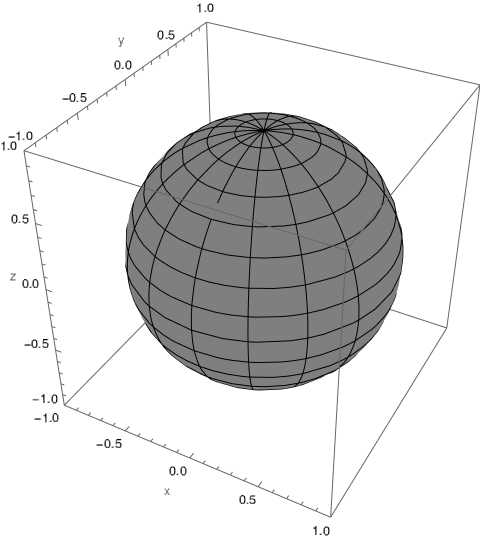
\includegraphics[width=0.6\linewidth]{../notes/log/maxent/figures/sphere_swapcontraction_t=0_z=0.9_p=0.9.png}
          \caption{$t=0$}
        \end{subfigure}%
        \begin{subfigure}{0.475\textwidth}
          \centering
          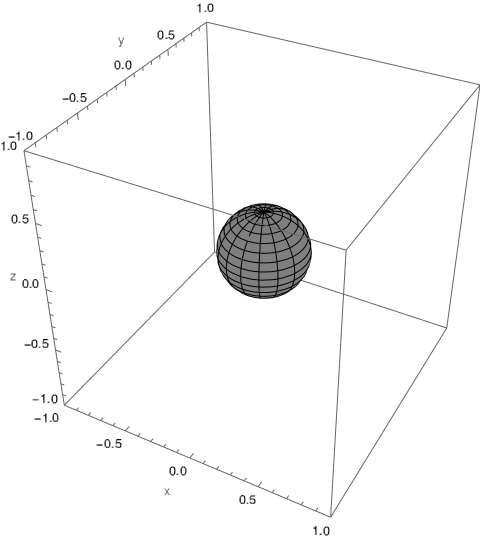
\includegraphics[width=0.6\linewidth]{../notes/log/maxent/figures/sphere_swapcontraction_t=1_z=0.9_p=0.9.png}
          \caption{$t=1$}
        \end{subfigure}
        \caption{Effect on the Bloch sphere if $r_{z}=0.9$, $p=0.9$. The dramatic size compression can be seen as a loss of information.}
        \label{fig:SWAPFactorSequence}
    \end{figure}
\end{frame}

\begin{frame}{SWAP gate}
    \begin{figure}[h!]
        \centering
        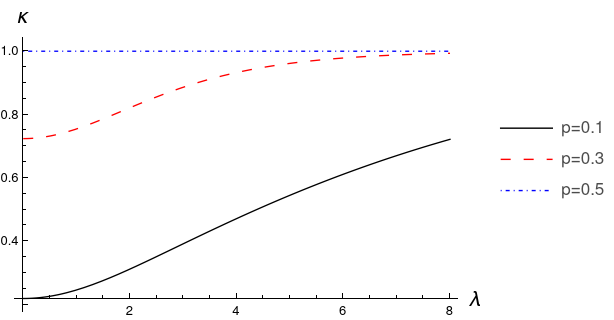
\includegraphics[width=0.6\linewidth]{../notes/log/maxent/figures/ContractionFactorSWAP_2D_lambda0to8.png}
        \caption{$\kappa_{1}$ as a function of $\lambda$, for different values of $p$.}
        \label{fig:SWAPFactor2D}
      \end{figure}
\end{frame}

\begin{frame}{Generalized SWAP gate}
    SWAP gate might be extended to an arbitrary time as $S^{t}$. In this case, 
    \begin{equation*}
        \kappa_{t}^{\rho}=\frac{((1-p)\cos^{2}{\frac{\pi t}{2}}+p\sin^{2}{\frac{\pi t}{2}})\tanh{\lambda p}+(p\cos^{2}{\frac{\pi t}{2}}+(1-p)\sin^{2}{\frac{\pi t}{2}})\tanh{\lambda (1-p)}}{
          p\tanh{\lambda p}+(1-p)\tanh{\lambda (1-p)}}.
      \end{equation*}
      In terms of the spin observable $\sigma_{z}$, evolution looks like
\begin{equation}
  \expval{\sigma_{z}(t)}=\kappa_{t}^{\rho}\expval{\sigma_{z}(0)}.
\end{equation}
Or, in terms of the probability of getting either $\ket{0}$ or $\ket{1}$ as
 \begin{align}
  \bra{0}\rho(t)\ket{0}=\frac{1}{2}(1+\kappa_{t}^{\rho}\expval{\sigma_{z}(0)}) && \bra{1}\rho(t)\ket{1}=\frac{1}{2}(1-\kappa_{t}^{\rho}\expval{\sigma_{z}(0)}),
 \end{align}
 where both non linearity and time dependency is contained inside the contraction factor $\kappa_{t}^{\rho}$. 
\end{frame}

\subsection{Separable dynamics}

\begin{frame}{Solution}
    Notice that, since $\rho_{max}$ state is of the form $\rho_{A}\otimes\rho_{B}$. The effective state might be written as 
    \begin{equation*}
        \rho=p\rho_{A}+\rho_{B}
    \end{equation*}
    Meaning that the evolution looks like
    \begin{equation*}
        \rho\xrightarrow{\mcU=U_{1}\otimes U_{2}} pU_{1}\rho_{A}U_{1}^{\dag}+(1-p)U_{2}\rho_{B}U_{2}^{\dag}
    \end{equation*}
    We recognize two special cases:
    \begin{align*}
        U_{2}=\Id&&U_{1}=U_{2}
    \end{align*}
\end{frame}

\begin{frame}{$U_{1}=U_{2}$}
    Quizá el caso más sencillo. La simetría de la unitaria permite factorizarla:
    \begin{align*}
    \CG{(U^{t}\otimes U^{t})\varrho_{max}(U^{t}\otimes U^{t})^{\dag}}&=p\frac{1}{Z_{1}}e^{-\lambda p U^{t}\sigma_{z}(U^t)^{\dag}}+(1-p)\frac{1}{Z_{2}}e^{-\lambda (1-p)U^{t}\sigma_{z}(U^t)^{\dag}}\\
    &=p\frac{1}{Z_{1}}U^{t}e^{-\lambda p \sigma_{z}}(U^t)^{\dag}+(1-p)\frac{1}{Z_{2}}U^{t}e^{-\lambda (1-p)\sigma_{z}}(U^t)^{\dag}\\
    &=U^{t}\qty(p\frac{1}{Z_{1}}e^{-\lambda p \sigma_{z}}+(1-p)\frac{1}{Z_{2}}e^{-\lambda (1-p)\sigma_{z}})(U^t)^{\dag}\\
    \end{align*}
    La dinámica efectiva tiene la forma:
    \begin{equation}
        \rho\xrightarrow{U\otimes U}U\rho U^{\dagger}
    \end{equation}
\end{frame}

\begin{frame}{$U_{2}=\Id$}
\begin{columns}
    \begin{column}{0.5\textwidth}
        Effective evolution looks like
        \begin{equation*}
            \rho\xrightarrow{\mcU=U_{1}\otimes U_{2}} pU_{1}\rho_{A}U_{1}^{\dag}+(1-p)\rho_{B}.
        \end{equation*}
        Using the Bloch vectors:
        \begin{equation*}
            r\hat{r}_{\rho}\xrightarrow{\mcU=U_{1}\otimes \Id}r_{A}O\hat{r}_{\rho}+r_{B}\hat{r}_{\rho}=O(r\hat{r}_{\rho}-r_{B}\hat{r}_{\rho})+r_{B}\hat{r}_{\rho}
        \end{equation*}
        i.e. $T^{-1}\circ R\circ T$, with $T$ a translation and $R$ a rotation. Note that $T$ depends on $\rho$. It is non-linear!
    \end{column}
    \begin{column}{0.5\textwidth}
        \begin{figure}[h!]
            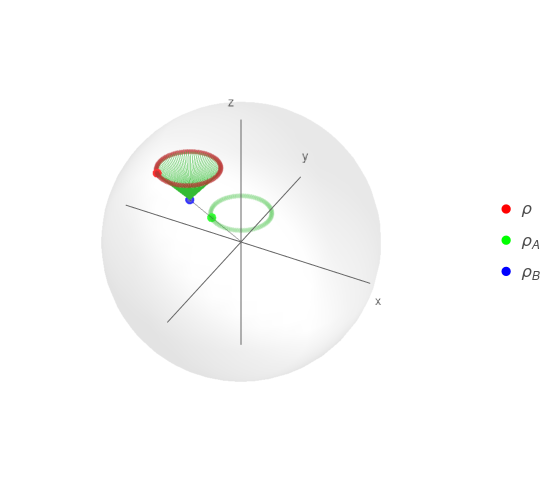
\includegraphics[width=0.8\linewidth]{../notes/log/maxent/figures/U1xU2_H1=sz_H2=Id_z=0.9_p=0.4_sequence.png}
            \caption{The effective state $\rho$ \textit{feels} the rotation induced by $U_{1}$}
            \label{fig:ZRot}
        \end{figure}
    \end{column}
\end{columns}
\end{frame}


\begin{frame}{The $(1-p)\rightarrow 0$ regime}
    Notice that, since $\rho_{max}$ state is of the form $\rho_{A}\otimes\rho_{B}$. The effective state might be written as 
    \begin{equation*}
        \rho=p\rho_{A}+\rho_{B}
    \end{equation*}
    Meaning that the evolution looks like
    \begin{equation*}
        \rho\xrightarrow{\mcU=U_{1}\otimes U_{2}} pU_{1}\rho_{A}U_{1}^{\dag}+(1-p)U_{2}\rho_{B}U_{2}^{\dag}
    \end{equation*}
    We recognize two special cases:
    \begin{align*}
        U_{2}=\Id&&U_{1}=U_{2}
    \end{align*}
\end{frame}

\subsection{Special Dynamics}

\begin{frame}{Ising Model}
Both $\rho(0)$ and $\rho(t)$ are aligned with the z axis.

Their $z$ coordinate is $r_{z}(0)$ and $r_{z}(1)$ respectively. 

The effect of the dynamics over a sphere of effective states with purity $r_z$ is to shrink it by a factor of $\frac{r_{z}(1)}{r_{z}(0)}$.
        \begin{equation*}
            \frac{r_{z}(1)}{r_{z}(0)}=\left(\frac{2 \sinh (\lambda )}{\sinh (\lambda )+(1-2 p) \sinh (\lambda -2 \lambda  p)}-1\right)
        \end{equation*}
        Note that the sphere will contract as a function of both $p$ and $r_{z}$
\end{frame}
\begin{frame}{Coarse pure states and the $p=\frac{1}{2}$ case}
    \begin{columns}
        \begin{column}{0.5\textwidth}
    From the previous results, if $p=\frac{1}{2}$:
    \begin{equation*}
        \Gamma_{t}^{\mcM,\rho}[\rho]=\rho \ \ \forall.
    \end{equation*}
The fuzzy map:
\begin{equation*}
    \mcF[\varrho]=\frac{1}{2}(\varrho+S\varrho S)=\mcF[S\varrho S] \ \ \forall \varrho.
\end{equation*}
This means that
\begin{equation*}
    \Gamma_{t}^{\mcA,\rho}[\rho]=\rho.
\end{equation*}
$\rho$ are fixed points if $p=\frac{1}{2}$.
        \end{column}
    \begin{column}{0.5\textwidth}
Let $\rho=\ket{\phi}\bra{\phi}$. Then the only compatible microscopic state is
$$\varrho=\rho\otimes\rho \ \ \Rightarrow \mcM[\rho]=\mcA[\rho]=\rho\otimes\rho  \ \ \forall p.$$
Because this state is invariant under particle permutation,
\begin{equation*}
    \Gamma_{t}^{\mcM,\rho}[\rho]=\rho \ \ \text{and} \ \ \Gamma_{t}^{\mcA,\rho}[\rho]=\rho.
\end{equation*}
Pure coarse states are fixed points under this kind of dynamics.
        \end{column}
    \end{columns}
\end{frame}

\begin{frame}[standout]
    \Huge\textsc{The end}
    
    \vfill
\end{frame}
\appendix

\begin{frame}{References}
\begin{thebibliography}{99}
\bibitem ONielsen, M. \& Chuang, L. (2010).\textit{Quantum Computation and Quantum Information}. Cambridge, United Kingdom: Cambridge University Press.
\bibitem OSilva, P. \& Concha, P. \& Vallejos, R. \& de Melo, F. (2020).\textit{Macro-to-micro quantum mapping and the emergence of nonlinearity}. PsyArXiv. DOI:10.1103/PhysRevA.103.052210
\end{thebibliography}
\end{frame}

\end{document}
